\section{Je reconnais les trois états physiques (3 poinst)}

Voici des récipients contenant des substances à l'état solide, à l'état liquide et à l'état gazeux.

\begin{questions}
	\question[3] En justifiant la réponse, indiquer l'état représenté dans chaque cas.
	%\begin{multicols}{2}
		
		\begin{center}
			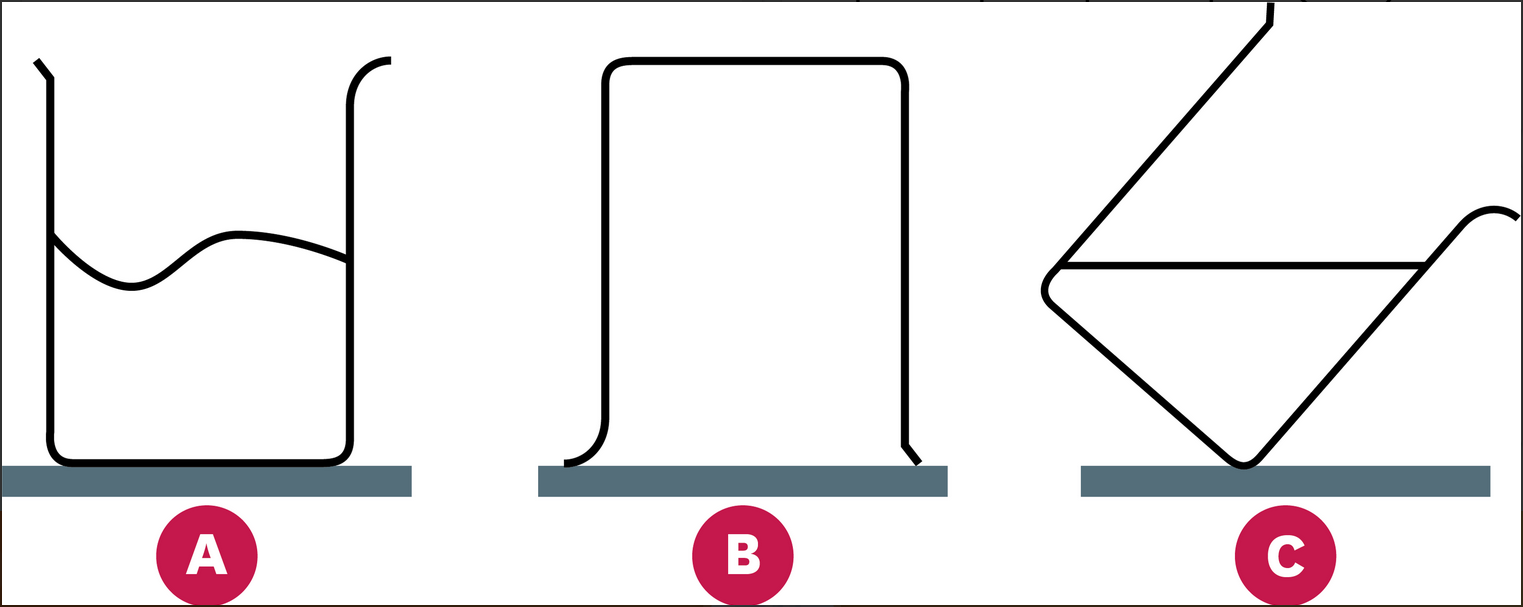
\includegraphics[scale=0.4]{img/reco1}
		\end{center}
	
		%\begin{center}
		%	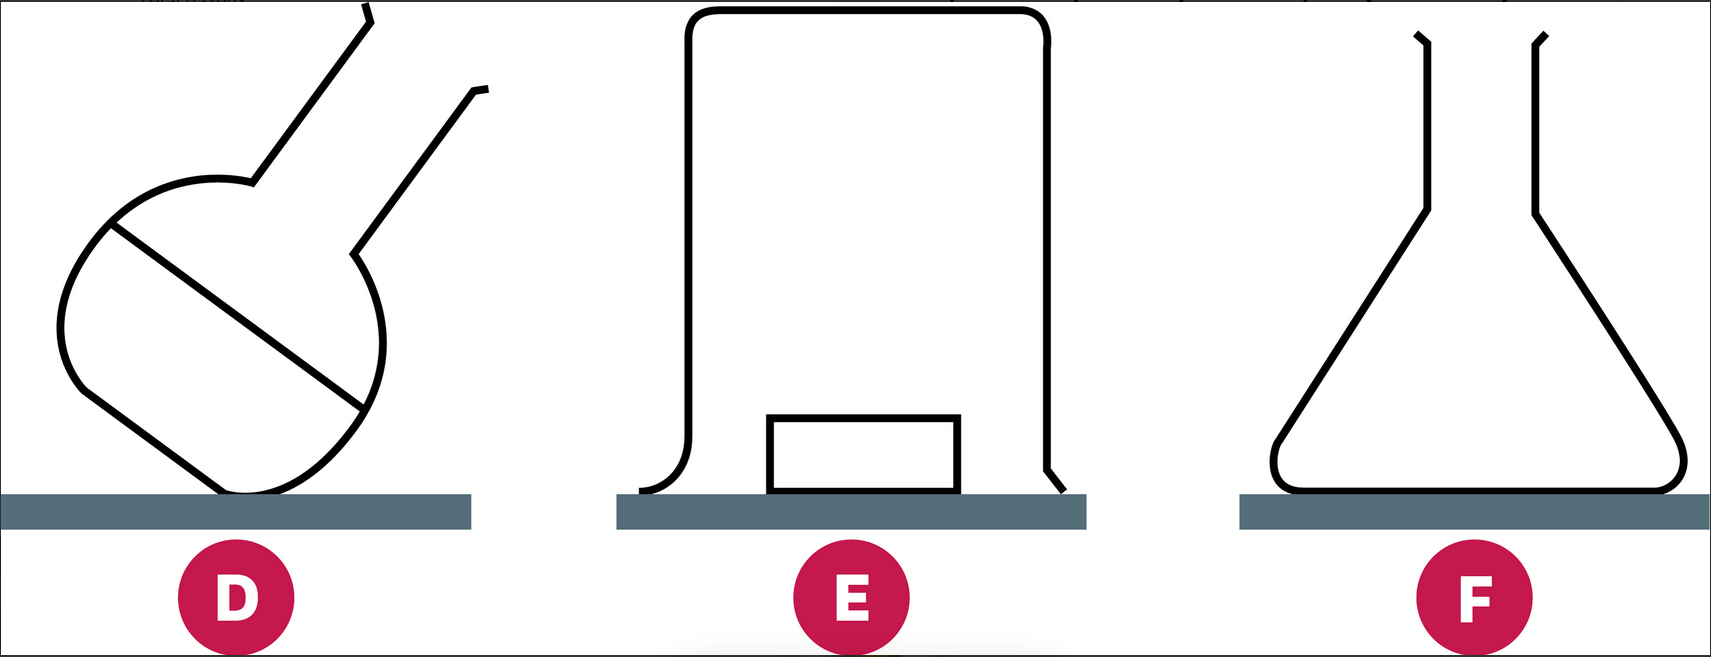
\includegraphics[scale=0.22]{img/reco2}
		%\end{center}

	%\end{multicols}
\end{questions}